
\documentclass[final]{beamer}



\usepackage[scale=0.8,size=a1]{beamerposter} % Use the beamerposter package for laying out the poster

\usetheme{confposter} % Use the confposter theme supplied with this template
\usepackage{multicol}
\setbeamercolor{block title}{fg=dblue,bg=white} % Colors of the block titles
\setbeamercolor{block body}{fg=black,bg=white} % Colors of the body of blocks
\setbeamercolor{block alerted title}{fg=white,bg=dblue!70} % Colors of the highlighted block titles
\setbeamercolor{block alerted body}{fg=black,bg=dblue!10} % Colors of the body of highlighted blocks
% Many more colors are available for use in beamerthemeconfposter.sty

%-----------------------------------------------------------
% Define the column widths and overall poster size
% To set effective sepwid, onecolwid and twocolwid values, first choose how many columns you want and how much separation you want between columns
% In this template, the separation width chosen is 0.024 of the paper width and a 4-column layout
% onecolwid should therefore be (1-(# of columns+1)*sepwid)/# of columns e.g. (1-(4+1)*0.024)/4 = 0.22
% Set twocolwid to be (2*onecolwid)+sepwid = 0.464
% Set threecolwid to be (3*onecolwid)+2*sepwid = 0.708

\newlength{\sepwid}
\newlength{\onecolwid}
\newlength{\twocolwid}
\newlength{\threecolwid}
\setlength{\paperwidth}{33.1in} % A0 width: 46.8in
\setlength{\paperheight}{23.4in} % A0 height: 33.1in
\setlength{\sepwid}{0.0\paperwidth} % Separation width (white space) between columns
\setlength{\onecolwid}{0.22\paperwidth} % Width of one column
\setlength{\twocolwid}{0.464\paperwidth} % Width of two columns
\setlength{\threecolwid}{0.708\paperwidth} % Width of three columns
\setlength{\topmargin}{-0.5in} % Reduce the top margin size
%-----------------------------------------------------------

\usepackage{graphicx}  % Required for including images

\usepackage{booktabs} % Top and bottom rules for tables
\usepackage{standalone} % to load standalone file (itkz picture for ex)
\usepackage{array} %finest gestion of tabular
\usepackage{algorithm,algorithmicx,algpseudocode}

%----------------------------------------------------------------------------------------
%	TITLE SECTION 
%----------------------------------------------------------------------------------------

%\title{Exploring the dynamic of cultural changes: A model to understand the amphorae production patterns in the Roman Empire} % Poster title
\title{New perspective on the study of variations in Amphorae production during the Roman Empire} % Poster title

\author{Maria Coto, Simon Carrignon and Xavier Rubio-Campillo} % Author(s)

\institute{Barcelona Supercomputing Center - University of Barcelona} % Institution(s)

%----------------------------------------------------------------------------------------

\begin{document}

\addtobeamertemplate{block end}{}{\vspace*{2ex}} % White space under blocks
\addtobeamertemplate{block alerted end}{}{\vspace*{2ex}} % White space under highlighted (alert) blocks

\setlength{\belowcaptionskip}{2ex} % White space under figures
\setlength\belowdisplayshortskip{2ex} % White space under equations

\begin{frame}[t] % The whole poster is enclosed in one beamer frame

\begin{columns}[t] % The whole poster consists of three major columns, the second of which is split into two columns twice - the [t] option aligns each column's content to the top

\begin{column}{\sepwid}\end{column} % Empty spacer column

\begin{column}{\onecolwid} % The first column


\begin{block}{Introduction}

Material culture variability allows to understand the interpretation of the change processes, focused on the production of olive oil amphorae (called Dressel 20) during the Roman Empire. \\
In particular, we want to identify changes on the pattern productions and if these changes were produced by economical and political reasons ~\cite{schillinger_differences_2016}. As
hypothesis, we think that making techniques processes were transmitted by vertical transmission based on the learning production techniques from master to disciple instead of horizontal transmission where this learning is done by workers with the same level. If this hypothesis is validated amphorae made in nearby workshops should share more traits than amphorae made from farthest workshops. Empirical studies and theoretical model were propose to test this hypothesis. 
\end{block}


\begin{block}{Dataset}


    We analysed a sample of 413 amphora shapes from 4 different workshops showed in the map \textbf{(fig.\ref{fig:betica})}.These workshops were selected from different sites of \emph{Baetica} province in order to know if morphometric distance was correlated with spatial distance. A set 90 samples from each workshop were used to create a database. 8 measures focused on the rim were taken from each amphorae sample. 

\begin{figure}
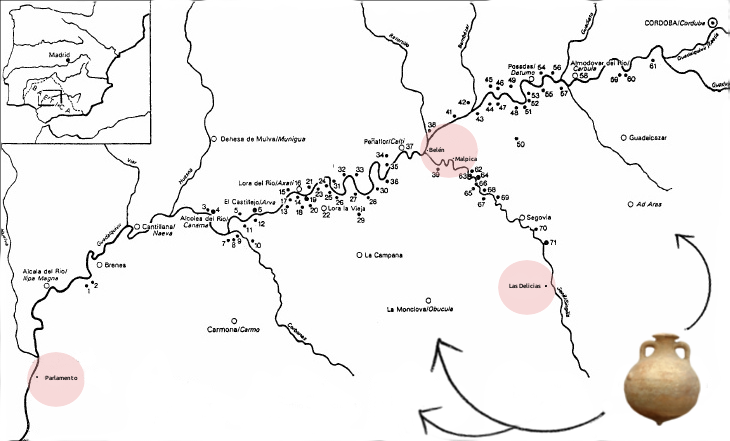
\includegraphics[width=0.7\linewidth]{images/fig1.png}
\caption{Pottery workshops were distributed along rivers Guadalquivir and Genil. Red circles belong to the workshops analysed}
\label{fig:betica}
\end{figure}


 \end{block}
\end{column} % End of the first column

%BEGIN THE SECOND COLUMN-------------------------------------------------
\begin{column}{\twocolwid}


\begin{block}{Multivariate analysis}
\begin{columns}[t,totalwidth=\twocolwid]



\begin{column}{\onecolwid} %first subcolumn left


{\textbf{Principal Component Analysis}} 
\justify

PCA was used to explore these metrical observations with the 8 measurement as variables. Results allow us to simplify the analysis by grouping the variance of the dataset. The first two principal components were chosen to see the significant differences among workshops. 

\vspace{1cm}
{\textbf{Results}}\\
\justify
Figure~\ref{fig:pca} shows that the closest workshops in space (Bel\'en and Malpica) produce more similar pottery traits than the farer workshops Parlamento and Las Delicias.


\end{column}

\begin{column}{\sepwid}\end{column} % Empty spacer column

\begin{column}{\onecolwid} %first subcolumn right


\begin{figure}
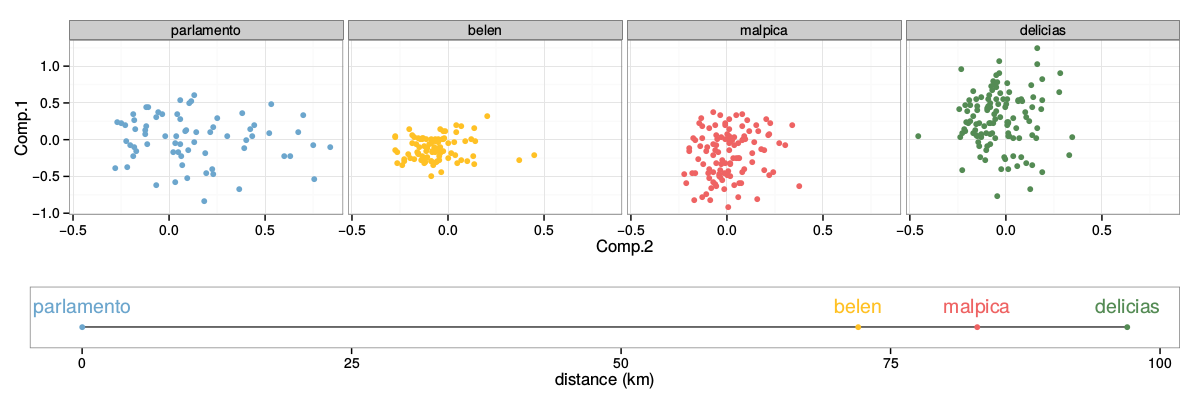
\includegraphics[width=0.6\linewidth]{images/fig2.png}
\caption{First and Second Principal Components for the analysed sample}
\label{fig:pca}
\end{figure}

\end{column}
 % End of the second column
\end{columns}

\end{block}

\begin{block}{Theoretical Exploration}

\begin{columns}[t,totalwidth=\twocolwid]

\begin{column}{1.025\onecolwid} %first subcolumn left
%on the left

{\textbf{Model}}\\
\justify
We propose a model implementing the Wright-Fisher view of Random Drift, where a fixed number of workshop produce a fixed amount of amphora during a certain time following a certain techniques. Every 100 time step each workshop have a certain probability to slightly modify their production technique (\emph{ie} the vertical tramsission) or to copy the one used by another workshop (\emph{the horizontal transmission}). 
	\begin{figure}
\begin{columns}
    \begin{column}{.6\textwidth}
	    \centering
	\resizebox{\textwidth}{!}{
	    \documentclass{standalone}

\begin{document}
    \begin{tikzpicture}[thick,scale=2]
		\coordinate (WS0) at (0,0);
		\coordinate (WS1) at (1,0);
		\coordinate (WS2) at (2,0);
		\coordinate (WS3) at (3,0);
		\draw[thick,-] (0,0) -- (3,0) node[anchor=north west] {};   
		\foreach \x in {0,1,2,3}
		\draw (\x cm,2pt) -- (\x cm,-2pt) node[anchor=north] {$WS_\x$};


		\draw [black,shorten <= 0.25cm, shorten >= 0.25cm, <->] (WS1) to[out=80,in=100,distance=1cm] node[above,font=\scriptsize]{knowledge transmission} (WS3); 


	\draw [black,shorten <= 0.7cm, shorten >= 0.7cm, <->] (WS0) to[out=-80,in=-100,distance=.75cm	]  node[font=\scriptsize,pos=.60	,above]{$T_{0 \rightarrow 1}$} (WS1);
	\draw [black,shorten <= 0.7cm, shorten >= 0.7cm, <->] (WS0) to[out=-80,in=-100,distance=1cm	]  node[font=\scriptsize,pos=.75	,above]{$T_{0 \rightarrow 2}$}(WS2);
	\draw [black,shorten <= 0.7cm, shorten >= 0.7cm, <->] (WS0) to[out=-80,in=-100,distance=1.25cm	]  node[font=\scriptsize,pos=.82		,above]{$T_{0 \rightarrow 3}$}(WS3);

    \end{tikzpicture}

\end{document}


}
	    \label{fig:mod}
    \end{column}
    \begin{column}{.4\textwidth}
	\begin{algorithmic}
	    \tiny
	    \State Model:
	    \Loop{$~step \in TimeSteps$}
	    \For{$i \in Pop$}
	    \State $AmphoraProduction(T^j)$
	    \If{$ (step \mod CulturalStep) = 0$}	
	    \State $Innovation(T^i)$
	    \State $CulturalTransmission(V)$
	    \EndIf
	    \EndFor
	    \EndLoop
	\end{algorithmic}
    \end{column}
\end{columns}

	    \caption{Schema (left) and pseudo-code (right) of the model }
	\end{figure}

{\textbf{Horizontal Transmission}}\\
\justify
To test the impact of horizontal transmission on the variation in production between the workshop we simplify the problem by focusin on the study of the variation of only one traits. We also introduce a penalties: workshops farer to $WS_0$ have lesser chance to make a cultural copy ($p=f(d)$ with $d$ the distance to $WS_0$)


\end{column}

%\begin{column}{.2\sepwid}\end{column} % Empty spacer column

\begin{column}{1.025\onecolwid} %first subcolumn right
\justify

{\textbf{Result}}\\
\justify
If the probability of horizontal transfer of knowledge between workshop is high the variation between the production is low. If the probability of cultural transfer is low, the variability is high, till it reaches its maximum where no horizontal transfer is allowed.

    \begin{figure}[h!]
    \centering
	\caption{Evolution of the variation of the mean of the observed measure between the workshops for different Horizontal Transmission penalities}
	%\begin{tabular}{m{.3\textwidth}m{.3\textwidth}m{.3\textwidth}}
    \begin{tabular}{ccc}
	     $f(d)=d$ & $f(d)=d^3$ & No Copy\\
	    
	    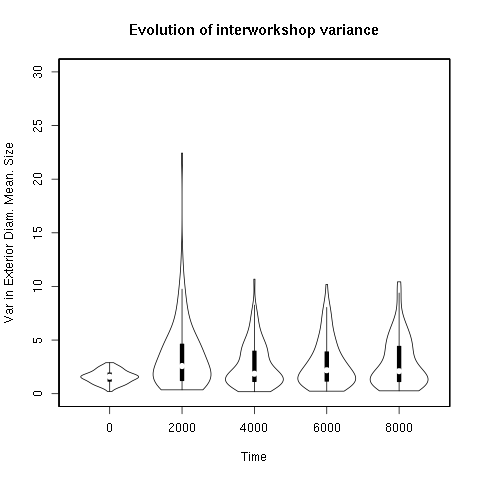
\includegraphics[height=.3\textwidth]{images/lineC.png}
	    &
	    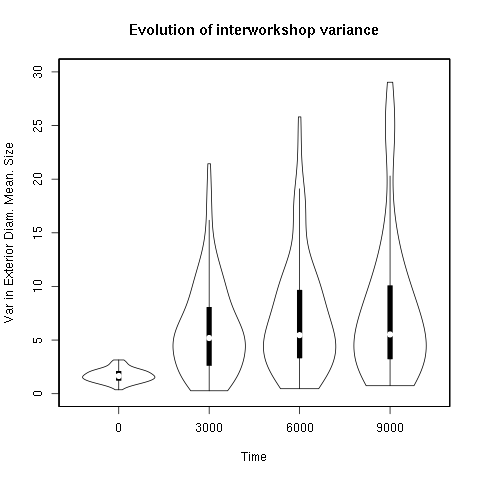
\includegraphics[height=.3\textwidth]{images/cubeC.png}
	    &
	    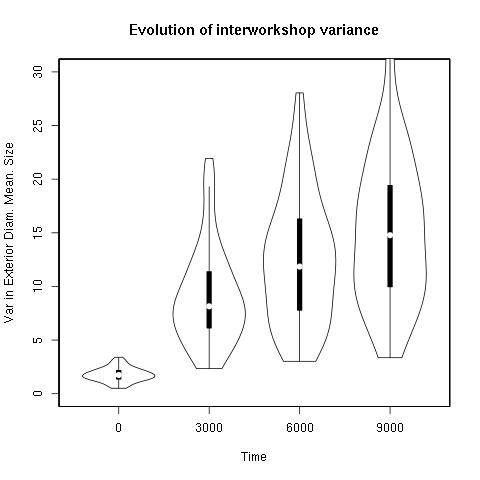
\includegraphics[height=.3\textwidth]{images/lineNC.png}\\
	\end{tabular}
	\label{fig:resmod}
    \end{figure}


    
\end{column}
 % End of the second column
\end{columns}

\end{block}
\end{column}

%BEGIN LAST COLUMN----------------------------------------------------

\begin{column}{\sepwid}\end{column} % Empty spacer column

\begin{column}{\onecolwid} % The third column

\begin{block}{Concluding Remarks}

Empirical studies identified a variation on the making techniques processes among pottery workshops. We observe that this variability is affected by the distance: amphorae made in nearby workshops with a minor spacial distance share more traits than amphorae made in pottery workshops farther. It suggests that the pottery techniques were learned from master to disciple instead of workers with the same level. 

The theoretical model support those claim as it shows that when introducing the possibility of horizontal transmission between the workshop the diversity of production quickly decrease.
\cite{lycett2015}
 
\end{block}

\begin{block}{References}

	\scriptsize
	\renewcommand{\refname}{\vspace{-0.5em}}
	//\bibliographystyle{abbrv}
	\bibliography{biblio}

\end{block}

%----------------------------------------------------------------------------------------
%	ACKNOWLEDGEMENTS
%----------------------------------------------------------------------------------------

\setbeamercolor{block title}{fg=dblue,bg=white} % Change the block title color

\begin{block}{Acknowledgements}

\small{\rmfamily{The Funding for this work was provided by the ERC Advanced Grant EPNet (340828)}}

\end{block}

%----------------------------------------------------------------------------------------
%	CONTACT INFORMATION
%----------------------------------------------------------------------------------------

\setbeamercolor{block alerted title}{fg=white,bg=dblue!70} % Change the alert block title colors
\setbeamercolor{block alerted body}{fg=black,bg=white} % Change the alert block body colors


\begin{center}
\begin{tabular}{ccc}

\includegraphics[width=0.4\linewidth]{images/epnet.png} & \hfill & 
\includegraphics[width=0.4\linewidth]{images/erc.png}
\end{tabular}
\end{center}

%----------------------------------------------------------------------------------------

\end{column} % End of the third column

\end{columns} % End of all the columns in the poster

\end{frame} % End of the enclosing frame

\end{document}
